%% Q1
Modern education is \textbf{child-centred (student-centred)}: the curriculum, methods and evaluation are organised around the learner's needs, interests, abilities and pace (Rousseau, Froebel, Dewey, Montessori). Education is meaningful only when it engages the learner actively.

%% Q2
In this paper the official key credits \textbf{social participation}. The project method, developed by W.~H.~Kilpatrick from Dewey's philosophy, has learners work together in groups on real-life, purposeful tasks. Learning thus takes place through cooperation and \emph{social participation}, in a lifelike social setting.
\tip{The same question in GSET Dec 2019 was keyed ``individualised engagement''. Both views are defensible, so always read the options carefully.}

%% Q3
\textbf{Continuous and Comprehensive Evaluation (CCE)} evaluates the \textbf{overall (scholastic and co-scholastic) development} of students \textbf{continuously} throughout the year. Continuous means regular formative and summative assessment. Comprehensive means covering cognitive, affective and psychomotor domains (academics, life skills, attitudes, co-curricular activities).

%% Q4
Audio-visual aids appeal to several senses at once. They make learners active participants, make the teacher's presentation more dynamic, and so make teaching more effective (``Seeing is believing''; Edgar Dale's Cone of Experience). All three statements are true.

%% Q5
A \textbf{diagnostic test} pinpoints the specific \textbf{weaknesses or learning difficulties} of a student in the content, and its purpose is to plan \textbf{remedial teaching}. Hence (A) and (C) both.
\why{Measuring overall scholastic achievement is the job of an \emph{achievement} test.}

%% Q6
The best teacher is concerned with the \textbf{all-round (holistic) development} of students: intellectual, emotional, social, moral and physical. Strict discipline, long hours or leadership training alone are narrower goals.

%% Q7
A \textbf{placebo} is an inert treatment (e.g.\ a sugar pill). The \textbf{placebo effect} is the \emph{positive} improvement that occurs simply because the subject believes a treatment is being given. In experiments a placebo group controls for this expectation effect.
\tip{A negative effect produced by negative expectations is called the \emph{nocebo} effect.}

%% Q8
In a factorial design the notation $2\times3\times2$ gives one number \emph{per independent variable} (factor), each number being the number of levels of that factor. Three numbers mean \textbf{three} variables (with $2\times3\times2=12$ treatment combinations).

%% Q9
A \textbf{true experimental design} has three features: manipulation of the independent variable, a control group, and \textbf{random assignment} (randomisation), which controls extraneous (external) variables.

%% Q10
\textbf{APA} is the \textbf{American Psychological Association}. Its \emph{Publication Manual} (7th ed., 2019) sets the ``APA style'' of referencing widely used in education and the social sciences.

%% Q11
Research ethics require \textbf{confidentiality}: information from respondents, especially sensitive information, must be kept private and used only for research purposes, with anonymity protected. Sharing it with family, colleagues or the public violates the informed-consent agreement.

%% Q12
In historical research, \textbf{external criticism} tests the \textbf{authenticity (genuineness or originality)} of a document or source: is it what it claims to be? (author, date, place, forgery). \textbf{Internal criticism} tests the \emph{credibility, accuracy and meaning of the content}.

%% Q13 ctx
\textbf{Read the following text and answer the questions 13 to 18.}\par\smallskip
The term `Street Children' is used to refer to children who live on the streets and are deprived of family care and protection. They live in abandoned buildings, containers, automobiles, parks or on street itself. A great deal has been written defining street children. The problem is that there are no precise categories but rather a continuum ranging from children who spend some time in the streets but basically live at home to those who live entirely in the streets and have no adult care. The street children live and work amidst trash, animals and open sewers. They are exposed to many diseases and are unlikely to receive any medical treatment as they cannot afford doctors or medicine. Other major problems of street children are: abuse, child labour, gender discrimination, homelessness and poverty. How can the civil society provide such children their basic constitutional right to health, freedom from violence and abuse is a big challenge.

%% Q13
The paragraph \textbf{describes} who street children are, where they live and the problems they face. It does not analyse causes, synthesise views or trace consequences, so it is \textbf{descriptive}.

%% Q14
The expression ``street children'' is a \textbf{coined term}: a phrase specially coined (by UNICEF and welfare agencies in the 1980s) to label children who live and work on the streets. The passage itself notes that ``a great deal has been written defining'' them, i.e.\ it is a label rather than a precise definition, concept or theoretical framework.

%% Q15
The opening sentence paints street children as those ``who live on the streets and are deprived of family care and protection'', i.e.\ children \textbf{without home and without parents} (family). The other options (child labour, disease, lack of rights) are consequences mentioned later.

%% Q16
According to the official key the main reason is that they \textbf{have no adult care}. With no one to look after them, they live amid trash and sewers and cannot get medical treatment.

%% Q17
Street children are ``\textbf{deprived of family care} and protection'' (first sentence). The other options contradict the passage.

%% Q18
The passage says they ``are unlikely to receive any medical treatment''. So ``they get medical treatment'' is \textbf{not correct}.

%% Q19
\textbf{Projection} is the perceptual tendency to attribute one's own thoughts, feelings or motives to others.
\why{Stereotyping judges a person by the group they belong to; the halo effect lets one good trait colour the overall impression.}

%% Q20
The interpersonal communication process in order:
\begin{center}
\begin{tikzpicture}[node distance=2mm,every node/.style={draw=brand,rounded corners,fill=soft,font=\scriptsize,minimum height=6mm}]
\node (a) {Sender (1)}; \node[right=of a] (b) {Encoding (6)}; \node[right=of b] (c) {Message (3)}; \node[right=of c] (d) {Channel (5)}; \node[right=of d] (e) {Receiver (2)}; \node[right=of e] (f) {Feedback (4)};
\foreach \x/\y in {a/b,b/c,c/d,d/e,e/f} \draw[-Stealth,brand] (\x)--(\y);
\end{tikzpicture}
\end{center}
The order is \textbf{1-6-3-5-2-4}, i.e.\ 163524.

%% Q21
The \textbf{message} is the content of communication: the information, idea or feeling that the sender wants to convey.

%% Q22
\textbf{Decoding}: the receiver interprets the symbols and converts them back into concepts and ideas.

%% Q23
The primary purpose of communication is to impart (share) \textbf{information}. Training, discipline and skills are specific outcomes that depend on communicating information.

%% Q24
The official key gives \textbf{written communication}: it is precise, permanent, verifiable, can reach many people and can be referred to repeatedly, which makes it the most reliable and effective form, especially in formal settings.

%% Q25
Each term is $n^2-1$: $1-1=0$, $4-1=3$, $9-1=8$, $16-1=15$, $25-1=24$, so next $36-1=\mathbf{35}$. (Differences: 3, 5, 7, 9, 11.)

%% Q26 fig
\begin{tabular}{|c|c|c|}\hline 0 & 2 & 4\\\hline 1 & 3 & 5\\\hline 7 & 9 & 11\\\hline 0 & 24 & ?\\\hline\end{tabular}

%% Q26
Work column by column: bottom $=$ top $\times$ (sum of the two middle numbers).
\[0\times(1+7)=0,\qquad 2\times(3+9)=24,\qquad 4\times(5+11)=\mathbf{64}\]

%% Q27
HEALTH $\rightarrow$ GSKZDG: \emph{reverse} the word (HTLAEH) and then move each letter \emph{one step back}: H$\rightarrow$G, T$\rightarrow$S, L$\rightarrow$K, A$\rightarrow$Z, E$\rightarrow$D, H$\rightarrow$G.
NORTH reversed is HTRON; one step back gives \textbf{GSQNM}.

%% Q28
Substituting: $14\times10+42\div2-8=140+21-8=\mathbf{153}$.

%% Q29
The key reads ``3 times more than'' as ``3 times''. Friend $=x$, person $=3x$, $4x=64\Rightarrow x=16$. The ages are \textbf{48 and 16}.

%% Q30
Add the two inequalities:
\[(A+B)+(B+C)>(C+D)+(A+D)\ \Rightarrow\ A+2B+C>A+C+2D\ \Rightarrow\ B>D\]
So \textbf{B $>$ D} is definite.

%% Q31
Aryabhata was a mathematician (and astronomer); \textbf{Varahamihira} (6th century, \emph{Pancha-Siddhantika}, \emph{Brihat-Samhita}) is best known as an \textbf{astronomer} and astrologer.

%% Q32 fig
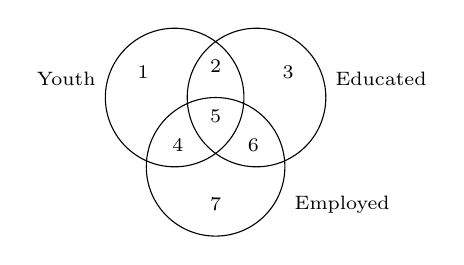
\begin{tikzpicture}[scale=0.8,font=\scriptsize]
\draw (0,0.5) circle(1.1); \draw (1.3,0.5) circle(1.1); \draw (0.65,-0.6) circle(1.1);
\node at (-0.5,0.9){1}; \node at (0.65,1.0){2}; \node at (1.8,0.9){3}; \node at (0.05,-0.25){4}; \node at (0.65,0.2){5}; \node at (1.25,-0.25){6}; \node at (0.65,-1.2){7};
\node[left] at (-1.1,0.8){Youth}; \node[right] at (2.4,0.8){Educated}; \node[right] at (1.75,-1.2){Employed};
\end{tikzpicture}

%% Q32
The required region is \emph{inside} Youth, \emph{inside} Employed and \emph{outside} Educated. Only region \textbf{4} satisfies all three conditions.
\why{5 is also educated, 6 is not youth, and 7 is employed only (not youth).}

%% Q33 q
The question below consists of two statements numbered I and II. You have to decide whether the data provided in the statements are sufficient to answer the question.\\
\textbf{How is Tanya related to the man in the photograph?}\\
(I) Man in the photograph is the only son of Tanya's grandfather.\\
(II) The man in photograph has no brothers or sisters and his father is Tanya's grandfather.

%% Q33 opts
Statement I alone is sufficient, II is not
Statement II alone is sufficient, I is not
Either statement I or II alone is sufficient
Both statements together are not sufficient

%% Q33
The official key holds that each statement alone establishes that the man is the only son of Tanya's grandfather, and therefore \textbf{Tanya's father}. (Strictly, Tanya could also be a daughter's child; the setters assume the paternal line.) Both statements give the same information, so \textbf{either I or II} alone suffices.

%% Q34 fig
\begin{tikzpicture}[scale=0.9,font=\scriptsize]
\coordinate (A) at (0,2.5); \coordinate (B) at (-2,0); \coordinate (C) at (2,0); \coordinate (D) at (0,0);
\coordinate (O) at (0,0.95); \coordinate (E) at ($(A)!0.449!(C)$);
\draw[thick] (A)--(B)--(C)--cycle; \draw[thick] (A)--(D); \draw[thick] (B)--(E); \draw[thick] (C)--(O);
\foreach \p/\pos in {A/above,B/left,C/right,D/below,O/left,E/right} \node[\pos] at (\p) {\p};
\end{tikzpicture}

%% Q34
Label the points as in the figure. The lines are AB, AC (through E), BC (through D), AD (through O), BE (through O) and CO. The triangles are:
\begin{center}\small
ABD, ABO, ABC, ABE, ADC, AOC, AOE, BOD, BOC, BEC, ODC, OEC
\end{center}
Total $=$ \textbf{12}.

%% Q35
Veena, sitar and guitar are \textbf{string} instruments; the \textbf{drum} is a percussion instrument, so it is the odd one out.

%% Q36 q
In the question below, there are two statements labelled as Assertion (A) and Reason (R).\\
\textbf{Assertion (A):} Indian President is the head of country.\\
\textbf{Reason (R):} Indian Parliament consists of the President, Lok Sabha and Rajya Sabha.

%% Q36
Both statements are true. The President is the constitutional Head of State (Art.~52--53), and Parliament consists of the President and the two Houses (Art.~79). But being part of Parliament is not \emph{why} the President is head of the country, so R does not explain A.

%% Q37 fig
\begin{tikzpicture}
\begin{axis}[ybar,width=10cm,height=4.4cm,bar width=13pt,ymin=0,ymax=25,
  symbolic x coords={Infrastructure,Transport,Advertisements,Taxes,R\&D,Salary,Interest on loans},xtick=data,
  x tick label style={rotate=30,anchor=east,font=\scriptsize},yticklabel style={font=\scriptsize},
  nodes near coords,every node near coord/.append style={font=\tiny},ylabel={\scriptsize Percent spent},
  axis x line*=bottom,axis y line*=left]
\addplot[fill=white,draw=ink] coordinates {(Infrastructure,20) (Transport,12.5) (Advertisements,15) (Taxes,10) (R\&D,5) (Salary,20) (Interest on loans,17.5)};
\end{axis}
\end{tikzpicture}

%% Q37 after
The expenditures on the interests on loans is by what percentage more than the expenditures on transport?

%% Q37
Interest on loans $=17.5\%$; transport $=12.5\%$.
\[\frac{17.5-12.5}{12.5}\times100=\frac{5}{12.5}\times100=\mathbf{40\%}\]

%% Q38 fig
\begin{tikzpicture}\pie[radius=1.4,text=pin,hide number,font=\scriptsize,color={brand!10,brand!30,brand!15,brand!40,brand!5}]{19.94/External Assistance 11{,}486,9.12/SPVS 5{,}252,8.52/Toll 4{,}910,10.42/Annuity 6{,}000,52/Market borrowing 29{,}952}\end{tikzpicture}

%% Q38 after
Total funds to be arranged for projects (phase II) $=$ Rs.~57,600 crores. The approximate ratio of funds to be arranged through toll and that through market borrowing is:

%% Q38
\[\frac{\text{Toll}}{\text{Market borrowing}}=\frac{4910}{29952}\approx\frac{1}{6.1}\approx\mathbf{1:6}\]

%% Q39
Gender (male/female) and mobile-phone use (user/non-user) are \textbf{categorical attributes}, i.e.\ qualities rather than measured quantities. The data are therefore \textbf{qualitative (nominal)}, typically analysed with a chi-square test of association.

%% Q40
\textbf{CSO} was the \textbf{Central Statistics Office} under the Ministry of Statistics and Programme Implementation (MoSPI), and the key's ``Central Statistical Office'' is this body. It compiled national accounts, GDP, IIP, CPI and so on. In 2019 it merged with the NSSO to form the \emph{National Statistical Office (NSO)}.

%% Q41
The official key gives \textbf{two pie charts}. Each chart shows how one category, PG students in one and PhD students in the other, is distributed among the ten institutions, i.e.\ each institution's share. (A multiple-bar diagram would be the choice for comparing absolute numbers side by side.)

%% Q42 fig
\small
\begin{tabular}{c c cc}\toprule
& & \multicolumn{2}{c}{\textbf{Males : Females}}\\\cmidrule(l){3-4}
\textbf{State} & \textbf{\% below poverty line} & \textbf{Below PL} & \textbf{Above PL}\\\midrule
P & 35 & 5 : 6 & 6 : 7\\ Q & 25 & 3 : 5 & 4 : 5\\ R & 24 & 1 : 2 & 2 : 3\\ S & 19 & 3 : 2 & 4 : 3\\ T & 15 & 5 : 3 & 3 : 2\\\bottomrule
\end{tabular}

%% Q42 after
What will be the number of females above poverty line in the state S if it is known that population of state S is 7 million?

%% Q42
State S: above poverty line $=100-19=81\%$ of 7 million $=5.67$ million.
Females : males above PL $=3:(4+3)$, so females $=\tfrac37\times5.67=\textbf{2.43 million}$.

%% Q43
\textbf{Instagram} was created by Kevin Systrom and Mike Krieger (launched October 2010) and acquired by Facebook in April 2012 for about US\$1 billion.

%% Q44
\textbf{NPTEL} is the \textbf{National Programme on Technology Enhanced Learning}, a joint initiative of the IITs and IISc funded by MHRD (since 2003). It offers online courses in engineering and science and is a SWAYAM national coordinator.

%% Q45
\textbf{URL} is \textbf{Uniform Resource Locator}, the web address of a resource, e.g.\ \texttt{https://www.example.com/index.html} (protocol, domain, path).

%% Q46
An \textbf{IP (Internet Protocol) address} is the unique numerical label assigned to each device on a network. IPv4 addresses are 32-bit (e.g.\ 192.168.1.1); IPv6 addresses are 128-bit.

%% Q47
\textbf{Ray Tomlinson} sent the first network e-mail on ARPANET in 1971 and chose the \textbf{``@''} symbol to separate the user name from the host name.

%% Q48
\textbf{HTML} is \textbf{HyperText Markup Language}, the standard language for creating web pages, devised by Tim Berners-Lee (1991).

%% Q49
\textbf{Jatropha curcas} is the main non-edible oilseed plant promoted for biodiesel in India (National Mission on Biodiesel, 2003). It grows on wasteland and does not compete with food crops.

%% Q50
The official key gives \textbf{increasing population}. A growing population drives higher consumption of resources, pollution, deforestation and emissions, and so underlies most global environmental problems. Climate change, rising temperature and melting icebergs are its \emph{consequences}.

%% Q51
Pesticides and chemical fertilisers applied to fields accumulate in the soil, alter soil chemistry, kill soil organisms and leave toxic residues. Their direct impact is \textbf{soil pollution}, though run-off can also pollute water.

%% Q52
\textbf{Tetraethyl lead (TEL)} was added to petrol as an \textbf{anti-knock agent}. It raises the octane rating and prevents premature ignition (knocking) in engines. It was banned because it emits toxic lead; India phased out leaded petrol by 2000.

%% Q53
Floods, volcanic eruptions and earthquakes are \textbf{natural} hazards. A \textbf{plane crash} is a \emph{man-made (technological)} disaster.

%% Q54
Deforestation, development of coastal zones and urbanisation disturb the natural environment. \textbf{Afforestation} (planting trees) \emph{restores} the environment, so it is the one that does not disturb it.

%% Q55
\textbf{Banasthali Vidyapith} (Rajasthan, founded 1935) is one of the largest residential \textbf{women's universities} in the world.
\why{Gujarat University, Gujarat Vidyapith and Sardar Patel University are co-educational.}

%% Q56
The \textbf{National Institute of Design (NID), Ahmedabad} was declared an \textbf{Institution of National Importance} by the NID Act, 2014.

%% Q57
The \textbf{National Council for Teacher Education (NCTE)} became a statutory body under the NCTE Act, 1993. It regulates norms, standards and quality in \textbf{teacher education} (B.Ed., D.El.Ed., M.Ed.).

%% Q58
\textbf{NEET} is the \textbf{National Eligibility cum Entrance Test} for admission to MBBS, BDS and allied courses, conducted by the NTA.

%% Q59
\textbf{NAAC} is the \textbf{National Assessment and Accreditation Council}, established in 1994 by UGC, Bengaluru.

%% Q60
In \textbf{NIRF 2017} (India Rankings), the \textbf{Indian Institute of Science, Bengaluru} was ranked first in the \emph{Overall} category.
